\begin{figure}[H]
    \begin{subfigure}{.49\textwidth}
        \centering
        \caption*{$u(x_1, x_2) = \min\{x_1, 3x_2\}$}
        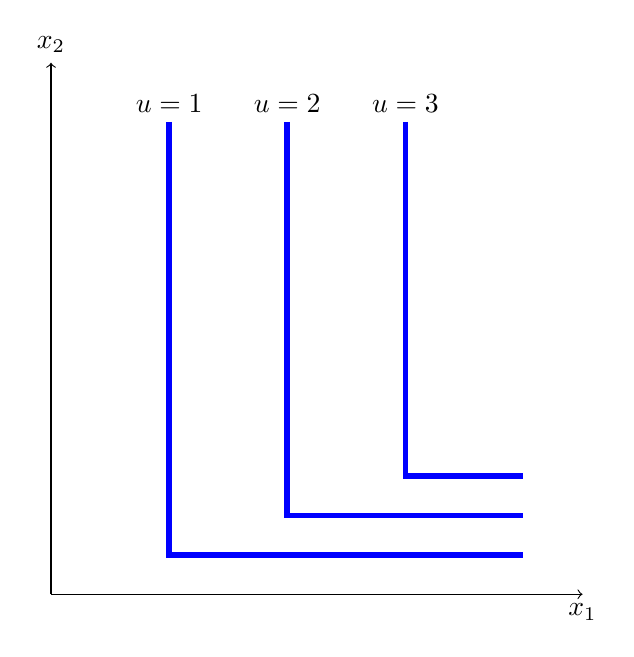
\begin{tikzpicture}[scale=1.5]
            \draw[->] (0, 0) -- (4.5, 0) node[below] {$x_1$};
            \draw[->] (0, 0) -- (0, 4.5) node[above] {$x_2$};
            \path[draw, blue, line width=2pt] (1,4) -- (1,1/3) -- (4,1/3);
            \path[draw, blue, line width=2pt] (2,4) -- (2,2/3) -- (4,2/3);
            \path[draw, blue, line width=2pt] (3,4) -- (3,1) -- (4,1);
            \node[above] at (1,4) {$u = 1$};
            \node[above] at (2,4) {$u = 2$};
            \node[above] at (3,4) {$u = 3$};
        \end{tikzpicture}
    \end{subfigure}
    \begin{subfigure}{.49\textwidth}
        \centering
        \caption*{$u(x_1, x_2) = 3\sqrt{x_1} + x_2$}
        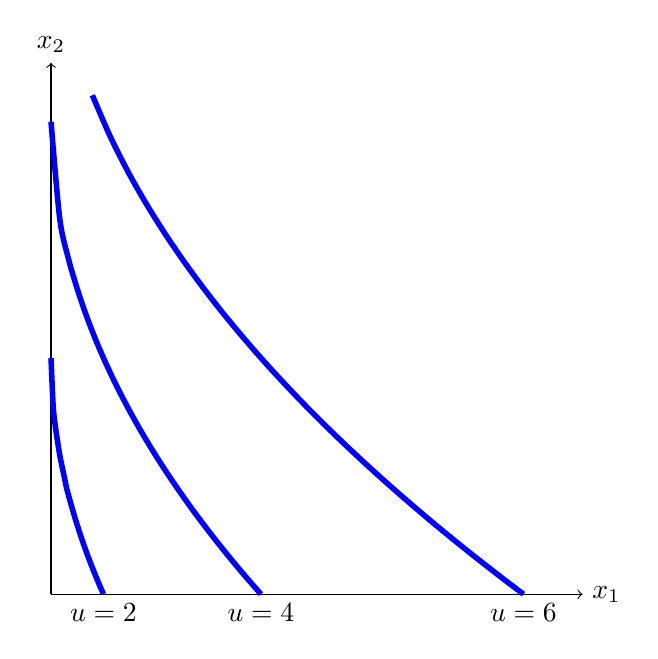
\begin{tikzpicture}[scale=1.5]
            \draw[->] (0, 0) -- (4.5, 0) node[right] {$x_1$};
            \draw[->] (0, 0) -- (0, 4.5) node[above] {$x_2$};
            \draw[domain=0:4/9, smooth, variable=\x, blue, line width=2pt] plot ({\x}, {2 - 3*\x^0.5});
            \draw[domain=0:16/9, smooth, variable=\x, blue, line width=2pt] plot ({\x}, {4 - 3*\x^0.5});
            \draw[domain=0.35:4, smooth, variable=\x, blue, line width=2pt] plot ({\x}, {6 - 3*\x^0.5});
            \node[below] at (4/9,0) {$u = 2$};
            \node[below] at (16/9,0) {$u = 4$};
            \node[below] at (4,0) {$u = 6$};
        \end{tikzpicture}
    \end{subfigure}
\end{figure}
